\documentclass[]{article}
\usepackage{lmodern}
\usepackage{amssymb,amsmath}
\usepackage{ifxetex,ifluatex}
\usepackage{fixltx2e} % provides \textsubscript
\ifnum 0\ifxetex 1\fi\ifluatex 1\fi=0 % if pdftex
  \usepackage[T1]{fontenc}
  \usepackage[utf8]{inputenc}
\else % if luatex or xelatex
  \ifxetex
    \usepackage{mathspec}
  \else
    \usepackage{fontspec}
  \fi
  \defaultfontfeatures{Ligatures=TeX,Scale=MatchLowercase}
\fi
% use upquote if available, for straight quotes in verbatim environments
\IfFileExists{upquote.sty}{\usepackage{upquote}}{}
% use microtype if available
\IfFileExists{microtype.sty}{%
\usepackage{microtype}
\UseMicrotypeSet[protrusion]{basicmath} % disable protrusion for tt fonts
}{}
\usepackage[margin=1in]{geometry}
\usepackage{hyperref}
\hypersetup{unicode=true,
            pdftitle={Aquatic Food Web Analysis},
            pdfauthor={Hannah M. Carroll and Derek D. Houston},
            pdfborder={0 0 0},
            breaklinks=true}
\urlstyle{same}  % don't use monospace font for urls
\usepackage{color}
\usepackage{fancyvrb}
\newcommand{\VerbBar}{|}
\newcommand{\VERB}{\Verb[commandchars=\\\{\}]}
\DefineVerbatimEnvironment{Highlighting}{Verbatim}{commandchars=\\\{\}}
% Add ',fontsize=\small' for more characters per line
\usepackage{framed}
\definecolor{shadecolor}{RGB}{248,248,248}
\newenvironment{Shaded}{\begin{snugshade}}{\end{snugshade}}
\newcommand{\KeywordTok}[1]{\textcolor[rgb]{0.13,0.29,0.53}{\textbf{#1}}}
\newcommand{\DataTypeTok}[1]{\textcolor[rgb]{0.13,0.29,0.53}{#1}}
\newcommand{\DecValTok}[1]{\textcolor[rgb]{0.00,0.00,0.81}{#1}}
\newcommand{\BaseNTok}[1]{\textcolor[rgb]{0.00,0.00,0.81}{#1}}
\newcommand{\FloatTok}[1]{\textcolor[rgb]{0.00,0.00,0.81}{#1}}
\newcommand{\ConstantTok}[1]{\textcolor[rgb]{0.00,0.00,0.00}{#1}}
\newcommand{\CharTok}[1]{\textcolor[rgb]{0.31,0.60,0.02}{#1}}
\newcommand{\SpecialCharTok}[1]{\textcolor[rgb]{0.00,0.00,0.00}{#1}}
\newcommand{\StringTok}[1]{\textcolor[rgb]{0.31,0.60,0.02}{#1}}
\newcommand{\VerbatimStringTok}[1]{\textcolor[rgb]{0.31,0.60,0.02}{#1}}
\newcommand{\SpecialStringTok}[1]{\textcolor[rgb]{0.31,0.60,0.02}{#1}}
\newcommand{\ImportTok}[1]{#1}
\newcommand{\CommentTok}[1]{\textcolor[rgb]{0.56,0.35,0.01}{\textit{#1}}}
\newcommand{\DocumentationTok}[1]{\textcolor[rgb]{0.56,0.35,0.01}{\textbf{\textit{#1}}}}
\newcommand{\AnnotationTok}[1]{\textcolor[rgb]{0.56,0.35,0.01}{\textbf{\textit{#1}}}}
\newcommand{\CommentVarTok}[1]{\textcolor[rgb]{0.56,0.35,0.01}{\textbf{\textit{#1}}}}
\newcommand{\OtherTok}[1]{\textcolor[rgb]{0.56,0.35,0.01}{#1}}
\newcommand{\FunctionTok}[1]{\textcolor[rgb]{0.00,0.00,0.00}{#1}}
\newcommand{\VariableTok}[1]{\textcolor[rgb]{0.00,0.00,0.00}{#1}}
\newcommand{\ControlFlowTok}[1]{\textcolor[rgb]{0.13,0.29,0.53}{\textbf{#1}}}
\newcommand{\OperatorTok}[1]{\textcolor[rgb]{0.81,0.36,0.00}{\textbf{#1}}}
\newcommand{\BuiltInTok}[1]{#1}
\newcommand{\ExtensionTok}[1]{#1}
\newcommand{\PreprocessorTok}[1]{\textcolor[rgb]{0.56,0.35,0.01}{\textit{#1}}}
\newcommand{\AttributeTok}[1]{\textcolor[rgb]{0.77,0.63,0.00}{#1}}
\newcommand{\RegionMarkerTok}[1]{#1}
\newcommand{\InformationTok}[1]{\textcolor[rgb]{0.56,0.35,0.01}{\textbf{\textit{#1}}}}
\newcommand{\WarningTok}[1]{\textcolor[rgb]{0.56,0.35,0.01}{\textbf{\textit{#1}}}}
\newcommand{\AlertTok}[1]{\textcolor[rgb]{0.94,0.16,0.16}{#1}}
\newcommand{\ErrorTok}[1]{\textcolor[rgb]{0.64,0.00,0.00}{\textbf{#1}}}
\newcommand{\NormalTok}[1]{#1}
\usepackage{graphicx,grffile}
\makeatletter
\def\maxwidth{\ifdim\Gin@nat@width>\linewidth\linewidth\else\Gin@nat@width\fi}
\def\maxheight{\ifdim\Gin@nat@height>\textheight\textheight\else\Gin@nat@height\fi}
\makeatother
% Scale images if necessary, so that they will not overflow the page
% margins by default, and it is still possible to overwrite the defaults
% using explicit options in \includegraphics[width, height, ...]{}
\setkeys{Gin}{width=\maxwidth,height=\maxheight,keepaspectratio}
\IfFileExists{parskip.sty}{%
\usepackage{parskip}
}{% else
\setlength{\parindent}{0pt}
\setlength{\parskip}{6pt plus 2pt minus 1pt}
}
\setlength{\emergencystretch}{3em}  % prevent overfull lines
\providecommand{\tightlist}{%
  \setlength{\itemsep}{0pt}\setlength{\parskip}{0pt}}
\setcounter{secnumdepth}{0}
% Redefines (sub)paragraphs to behave more like sections
\ifx\paragraph\undefined\else
\let\oldparagraph\paragraph
\renewcommand{\paragraph}[1]{\oldparagraph{#1}\mbox{}}
\fi
\ifx\subparagraph\undefined\else
\let\oldsubparagraph\subparagraph
\renewcommand{\subparagraph}[1]{\oldsubparagraph{#1}\mbox{}}
\fi

%%% Use protect on footnotes to avoid problems with footnotes in titles
\let\rmarkdownfootnote\footnote%
\def\footnote{\protect\rmarkdownfootnote}

%%% Change title format to be more compact
\usepackage{titling}

% Create subtitle command for use in maketitle
\newcommand{\subtitle}[1]{
  \posttitle{
    \begin{center}\large#1\end{center}
    }
}

\setlength{\droptitle}{-2em}

  \title{Aquatic Food Web Analysis}
    \pretitle{\vspace{\droptitle}\centering\huge}
  \posttitle{\par}
    \author{Hannah M. Carroll and Derek D. Houston}
    \preauthor{\centering\large\emph}
  \postauthor{\par}
      \predate{\centering\large\emph}
  \postdate{\par}
    \date{April 17th, 2019}


\begin{document}
\maketitle

\begin{itemize}
\item
  This is an R Notebook, which is written in RMarkdown format. Code is
  run inline in a code chunk, and the output appears directly below it.
\item
  Today's exercise will walk you through analysis of your aquatic
  isotope data and show you how to build a food web.
\item
  When typing into an R Notebook, you don't need to use \# to mark text
  as a comment, unless you're in an code chunk.
\end{itemize}

\begin{center}\rule{0.5\linewidth}{\linethickness}\end{center}

Your name:

\begin{center}\rule{0.5\linewidth}{\linethickness}\end{center}

A code chunk is standalone code that runs within the window. Code chunks
begin with \texttt{\{r\}\ and\ end\ with}

Try executing this chunk by clicking the \emph{Run} button (green right
arrow) within the chunk or by placing your cursor inside it and pressing
\emph{Ctrl+Shift+Enter}.

\begin{Shaded}
\begin{Highlighting}[]
\CommentTok{# Set your working directory by choosing Session from the menu at the top, then Set Working Directory -> To Source File Location}

\CommentTok{# (1pt) Write the command getwd() on the line below and run it to find out what your working directory is.}
\KeywordTok{getwd}\NormalTok{()}
\end{Highlighting}
\end{Shaded}

\begin{verbatim}
## [1] "C:/Users/Hannah/Documents/Research/For Derek/Derek teaching/Aquatic isotopes"
\end{verbatim}

\begin{center}\rule{0.5\linewidth}{\linethickness}\end{center}

We will start by loading required packages

\begin{Shaded}
\begin{Highlighting}[]
\NormalTok{packages <-}\StringTok{ }\KeywordTok{c}\NormalTok{(}\StringTok{"readxl"}\NormalTok{, }\StringTok{"ggplot2"}\NormalTok{, }\StringTok{"cluster"}\NormalTok{, }\StringTok{"factoextra"}\NormalTok{, }\StringTok{"tRophicPosition"}\NormalTok{, }\StringTok{"viridis"}\NormalTok{) }\CommentTok{# Make a list of required packages}

\CommentTok{# (1pt) How many packages are in our list?}
\CommentTok{# 6}

\NormalTok{new.packages <-}\StringTok{ }\NormalTok{packages[}\OperatorTok{!}\NormalTok{(packages }\OperatorTok\StringTok{ }\KeywordTok{installed.packages}\NormalTok{()[,}\StringTok{"Package"}\NormalTok{])] }\CommentTok{# Which ones haven't been installed yet?}

\CommentTok{# (1pt) What new packages are we installing?}
\CommentTok{# This will vary. Probably 3-5.}

\ControlFlowTok{if}\NormalTok{(}\KeywordTok{length}\NormalTok{(new.packages)) }\KeywordTok{install.packages}\NormalTok{(new.packages) }\CommentTok{# Install any that are missing}

\KeywordTok{lapply}\NormalTok{(packages, library, }\DataTypeTok{character.only =} \OtherTok{TRUE}\NormalTok{) }\CommentTok{# Load packages into memory for use}
\end{Highlighting}
\end{Shaded}

\begin{verbatim}
## Warning: package 'ggplot2' was built under R version 3.5.3
\end{verbatim}

\begin{verbatim}
## Warning: package 'factoextra' was built under R version 3.5.3
\end{verbatim}

\begin{verbatim}
## Welcome! Related Books: `Practical Guide To Cluster Analysis in R` at https://goo.gl/13EFCZ
\end{verbatim}

\begin{verbatim}
## Warning: package 'tRophicPosition' was built under R version 3.5.3
\end{verbatim}

\begin{verbatim}
## This is tRophicPosition 0.7.7
\end{verbatim}

\begin{verbatim}
## Loading required package: viridisLite
\end{verbatim}

\begin{verbatim}
## [[1]]
## [1] "readxl"    "stats"     "graphics"  "grDevices" "utils"     "datasets" 
## [7] "methods"   "base"     
## 
## [[2]]
## [1] "ggplot2"   "readxl"    "stats"     "graphics"  "grDevices" "utils"    
## [7] "datasets"  "methods"   "base"     
## 
## [[3]]
##  [1] "cluster"   "ggplot2"   "readxl"    "stats"     "graphics" 
##  [6] "grDevices" "utils"     "datasets"  "methods"   "base"     
## 
## [[4]]
##  [1] "factoextra" "cluster"    "ggplot2"    "readxl"     "stats"     
##  [6] "graphics"   "grDevices"  "utils"      "datasets"   "methods"   
## [11] "base"      
## 
## [[5]]
##  [1] "tRophicPosition" "factoextra"      "cluster"        
##  [4] "ggplot2"         "readxl"          "stats"          
##  [7] "graphics"        "grDevices"       "utils"          
## [10] "datasets"        "methods"         "base"           
## 
## [[6]]
##  [1] "viridis"         "viridisLite"     "tRophicPosition"
##  [4] "factoextra"      "cluster"         "ggplot2"        
##  [7] "readxl"          "stats"           "graphics"       
## [10] "grDevices"       "utils"           "datasets"       
## [13] "methods"         "base"
\end{verbatim}

Now, read in your dataset

\begin{Shaded}
\begin{Highlighting}[]
\NormalTok{isotope.data <-}\StringTok{ }\KeywordTok{read_excel}\NormalTok{(}\StringTok{"2019_EA_Houston_class project.xlsx"}\NormalTok{)}

\CommentTok{# The dataset should now appear in your global environment (top right)}

\CommentTok{# (1pt) How many observations are there?}
\CommentTok{# 19}

\CommentTok{# (1pt) How many variables are there?}
\CommentTok{# 8}
\end{Highlighting}
\end{Shaded}

\begin{center}\rule{0.5\linewidth}{\linethickness}\end{center}

Next, make a simple dual isotope plot of your data. Error bars are
plotted for both the x and y axes.

\begin{Shaded}
\begin{Highlighting}[]
\KeywordTok{ggplot}\NormalTok{(}\DataTypeTok{data=}\NormalTok{isotope.data, }\KeywordTok{aes}\NormalTok{(}\DataTypeTok{x=}\StringTok{`}\DataTypeTok{corrected d13C (VPDB)}\StringTok{`}\NormalTok{, }\DataTypeTok{y=}\StringTok{`}\DataTypeTok{corrected d15N (Air)}\StringTok{`}\NormalTok{, }\DataTypeTok{color=}\NormalTok{Trophic)) }\OperatorTok{+}\StringTok{ }
\StringTok{  }\KeywordTok{geom_errorbar}\NormalTok{(}\KeywordTok{aes}\NormalTok{(}\DataTypeTok{ymin=}\NormalTok{(}\StringTok{`}\DataTypeTok{corrected d15N (Air)}\StringTok{`}\OperatorTok{-}\FloatTok{0.09}\NormalTok{), }\DataTypeTok{ymax=}\NormalTok{(}\StringTok{`}\DataTypeTok{corrected d15N (Air)}\StringTok{`}\OperatorTok{+}\FloatTok{0.09}\NormalTok{))) }\OperatorTok{+}\StringTok{ }
\StringTok{  }\KeywordTok{geom_errorbarh}\NormalTok{(}\KeywordTok{aes}\NormalTok{(}\DataTypeTok{xmin=}\NormalTok{(}\StringTok{`}\DataTypeTok{corrected d13C (VPDB)}\StringTok{`}\OperatorTok{-}\FloatTok{0.11}\NormalTok{), }\DataTypeTok{xmax=}\NormalTok{(}\StringTok{`}\DataTypeTok{corrected d13C (VPDB)}\StringTok{`}\OperatorTok{+}\FloatTok{0.11}\NormalTok{))) }\OperatorTok{+}\StringTok{ }
\StringTok{  }\KeywordTok{geom_point}\NormalTok{() }\OperatorTok{+}
\StringTok{  }\KeywordTok{geom_text}\NormalTok{(}\KeywordTok{aes}\NormalTok{(}\DataTypeTok{label=}\NormalTok{ID, }\DataTypeTok{hjust=}\FloatTok{0.5}\NormalTok{), }\DataTypeTok{check_overlap =} \OtherTok{FALSE}\NormalTok{, }\DataTypeTok{hjust =} \DecValTok{0}\NormalTok{, }\DataTypeTok{nudge_x =} \FloatTok{0.2}\NormalTok{) }\OperatorTok{+}\StringTok{ }\KeywordTok{xlim}\NormalTok{(}\OperatorTok{-}\DecValTok{30}\NormalTok{,}\OperatorTok{-}\DecValTok{17}\NormalTok{) }\OperatorTok{+}
\StringTok{  }\KeywordTok{scale_color_viridis_d}\NormalTok{(}\DataTypeTok{name=}\StringTok{"Trophic Position"}\NormalTok{, }\DataTypeTok{breaks=}\KeywordTok{c}\NormalTok{(}\StringTok{"Apex"}\NormalTok{, }\StringTok{"Sec Consumer"}\NormalTok{, }\StringTok{"Herbivore"}\NormalTok{, }\StringTok{"Detritivore"}\NormalTok{,}
                                                          \StringTok{"HerbivoreDetritivore"}\NormalTok{, }\StringTok{"Primary Producer"}\NormalTok{, }\StringTok{"Detritus"}\NormalTok{)) }\OperatorTok{+}\StringTok{ }\KeywordTok{theme_bw}\NormalTok{()}
\end{Highlighting}
\end{Shaded}

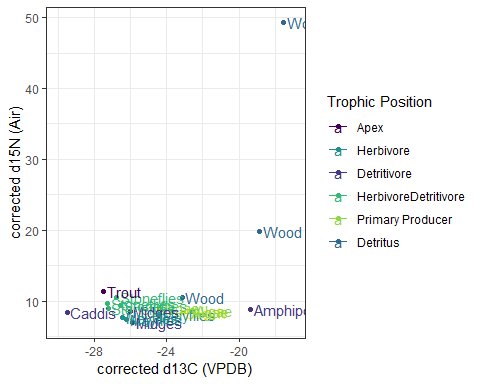
\includegraphics{Aquatic_food_web_files/figure-latex/unnamed-chunk-4-1.pdf}

(2pts) Describe what you see in the plot you just created. Which members
of the community group together and which do not? Do you notice anything
that doesn't seem to fit with the rest of the community?

(Answers will vary, but should note grouping of like creatures, wood off
by itself, etc.)

\begin{center}\rule{0.5\linewidth}{\linethickness}\end{center}

Now we'll determine whether there are outliers in either d13C or d15N.

\begin{Shaded}
\begin{Highlighting}[]
\KeywordTok{hist}\NormalTok{(isotope.data}\OperatorTok{$}\StringTok{`}\DataTypeTok{corrected d13C (VPDB)}\StringTok{`}\NormalTok{)}
\end{Highlighting}
\end{Shaded}

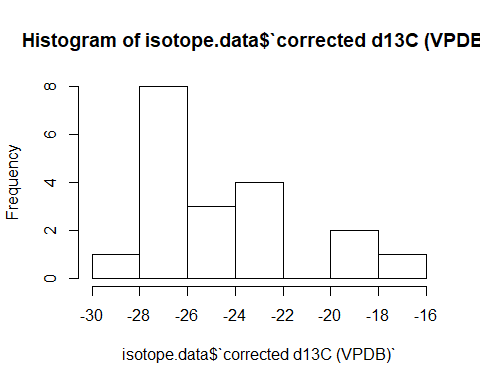
\includegraphics{Aquatic_food_web_files/figure-latex/unnamed-chunk-5-1.pdf}

\begin{Shaded}
\begin{Highlighting}[]
\CommentTok{# (1pt) Describe the distribution of our d13C data. Are they right skewed, left skewed, bimodal, or normally distributed?}
\CommentTok{# Right skewed}
\end{Highlighting}
\end{Shaded}

\begin{center}\rule{0.5\linewidth}{\linethickness}\end{center}

\begin{Shaded}
\begin{Highlighting}[]
\KeywordTok{hist}\NormalTok{(isotope.data}\OperatorTok{$}\StringTok{`}\DataTypeTok{corrected d15N (Air)}\StringTok{`}\NormalTok{)}
\end{Highlighting}
\end{Shaded}

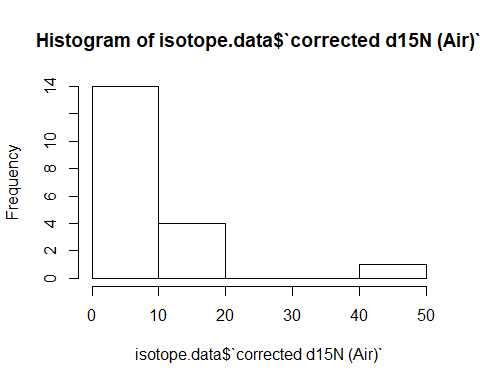
\includegraphics{Aquatic_food_web_files/figure-latex/unnamed-chunk-6-1.pdf}

\begin{Shaded}
\begin{Highlighting}[]
\CommentTok{# (1pt) Describe the distribution of our d15N data. Are they right skewed, left skewed, bimodal, or normally distributed?}
\CommentTok{# Right skewed}
\end{Highlighting}
\end{Shaded}

\begin{center}\rule{0.5\linewidth}{\linethickness}\end{center}

We can tell from our histograms that some of the observations in our
d15N dataset are true outliers. We need to remove those to complete our
analyses.

\begin{Shaded}
\begin{Highlighting}[]
\CommentTok{# The command below creates a new dataset by taking our original data and keeping only those rows where the value of d15N is less than 40. }

\NormalTok{iso.data.clean <-}\StringTok{ }\NormalTok{isotope.data[isotope.data}\OperatorTok{$}\StringTok{`}\DataTypeTok{corrected d15N (Air)}\StringTok{`} \OperatorTok{<}\StringTok{ }\DecValTok{40}\NormalTok{,]}

\CommentTok{# (1pt) Why was this chosen as the cutoff point?}
\CommentTok{# There is a big gap in the data and this looks an outlier.}

\CommentTok{# (1pt) How many observations does our new dataset contain?}
\CommentTok{# 18}

\CommentTok{# (1pt) How many variables?}
\CommentTok{# 8}
\end{Highlighting}
\end{Shaded}

\begin{Shaded}
\begin{Highlighting}[]
\CommentTok{# Now we plot the cleaned data:}

\KeywordTok{hist}\NormalTok{(iso.data.clean}\OperatorTok{$}\StringTok{`}\DataTypeTok{corrected d15N (Air)}\StringTok{`}\NormalTok{)}
\end{Highlighting}
\end{Shaded}

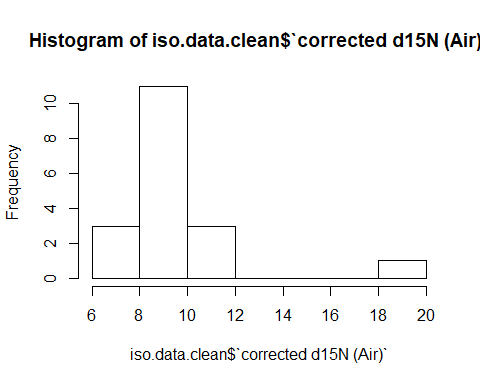
\includegraphics{Aquatic_food_web_files/figure-latex/unnamed-chunk-8-1.pdf}

It looks a lot better. However, we still have one outlier.

\begin{center}\rule{0.5\linewidth}{\linethickness}\end{center}

(2pts) Complete the line of code below to remove it, using what we did
before as a guide:

\begin{Shaded}
\begin{Highlighting}[]
\NormalTok{iso.data.clean2 <-}\StringTok{ }\NormalTok{isotope.data[isotope.data}\OperatorTok{$}\StringTok{`}\DataTypeTok{corrected d15N (Air)}\StringTok{`} \OperatorTok{<}\StringTok{ }\DecValTok{18}\NormalTok{,]}

\CommentTok{# iso.data.clean2 <- isotope.data[isotope.data$`corrected d15N (Air)` < 18,]}
\end{Highlighting}
\end{Shaded}

\begin{Shaded}
\begin{Highlighting}[]
\CommentTok{# Now plot the histogram:}

\KeywordTok{hist}\NormalTok{(iso.data.clean2}\OperatorTok{$}\StringTok{`}\DataTypeTok{corrected d15N (Air)}\StringTok{`}\NormalTok{)}
\end{Highlighting}
\end{Shaded}

\includegraphics{Aquatic_food_web_files/figure-latex/unnamed-chunk-10-1.pdf}

\begin{Shaded}
\begin{Highlighting}[]
\CommentTok{# (1pt) What kind of distribution do we have now? Is it right skewed, left skewed, bimodal, or normal?}
\CommentTok{# Normal}
\end{Highlighting}
\end{Shaded}

\begin{center}\rule{0.5\linewidth}{\linethickness}\end{center}

Now we will plot the dataset with our two outliers removed. You can see
the errorbars more clearly on this plot.

\begin{Shaded}
\begin{Highlighting}[]
\KeywordTok{ggplot}\NormalTok{(}\DataTypeTok{data=}\NormalTok{iso.data.clean2, }\KeywordTok{aes}\NormalTok{(}\DataTypeTok{x=}\StringTok{`}\DataTypeTok{corrected d13C (VPDB)}\StringTok{`}\NormalTok{, }\DataTypeTok{y=}\StringTok{`}\DataTypeTok{corrected d15N (Air)}\StringTok{`}\NormalTok{, }\DataTypeTok{color=}\NormalTok{Trophic)) }\OperatorTok{+}\StringTok{ }
\StringTok{  }\KeywordTok{geom_errorbar}\NormalTok{(}\KeywordTok{aes}\NormalTok{(}\DataTypeTok{ymin=}\NormalTok{(}\StringTok{`}\DataTypeTok{corrected d15N (Air)}\StringTok{`}\OperatorTok{-}\FloatTok{0.09}\NormalTok{), }\DataTypeTok{ymax=}\NormalTok{(}\StringTok{`}\DataTypeTok{corrected d15N (Air)}\StringTok{`}\OperatorTok{+}\FloatTok{0.09}\NormalTok{))) }\OperatorTok{+}\StringTok{ }
\StringTok{  }\KeywordTok{geom_errorbarh}\NormalTok{(}\KeywordTok{aes}\NormalTok{(}\DataTypeTok{xmin=}\NormalTok{(}\StringTok{`}\DataTypeTok{corrected d13C (VPDB)}\StringTok{`}\OperatorTok{-}\FloatTok{0.11}\NormalTok{), }\DataTypeTok{xmax=}\NormalTok{(}\StringTok{`}\DataTypeTok{corrected d13C (VPDB)}\StringTok{`}\OperatorTok{+}\FloatTok{0.11}\NormalTok{))) }\OperatorTok{+}\StringTok{ }
\StringTok{  }\KeywordTok{geom_point}\NormalTok{() }\OperatorTok{+}
\StringTok{  }\KeywordTok{geom_text}\NormalTok{(}\KeywordTok{aes}\NormalTok{(}\DataTypeTok{label=}\NormalTok{ID, }\DataTypeTok{hjust=}\FloatTok{0.5}\NormalTok{), }\DataTypeTok{check_overlap =} \OtherTok{FALSE}\NormalTok{, }\DataTypeTok{hjust =} \DecValTok{0}\NormalTok{, }\DataTypeTok{nudge_x =} \FloatTok{0.2}\NormalTok{) }\OperatorTok{+}\StringTok{ }\KeywordTok{xlim}\NormalTok{(}\OperatorTok{-}\DecValTok{30}\NormalTok{,}\OperatorTok{-}\DecValTok{17}\NormalTok{) }\OperatorTok{+}
\StringTok{  }\KeywordTok{scale_color_viridis_d}\NormalTok{(}\DataTypeTok{name=}\StringTok{"Trophic Position"}\NormalTok{, }\DataTypeTok{breaks=}\KeywordTok{c}\NormalTok{(}\StringTok{"Apex"}\NormalTok{, }\StringTok{"Sec Consumer"}\NormalTok{, }\StringTok{"Herbivore"}\NormalTok{, }\StringTok{"Detritivore"}\NormalTok{,}
                                                          \StringTok{"HerbivoreDetritivore"}\NormalTok{, }\StringTok{"Primary Producer"}\NormalTok{, }\StringTok{"Detritus"}\NormalTok{)) }\OperatorTok{+}\StringTok{ }\KeywordTok{theme_bw}\NormalTok{()}
\end{Highlighting}
\end{Shaded}

\includegraphics{Aquatic_food_web_files/figure-latex/unnamed-chunk-11-1.pdf}

(1pt) Describe what you see in the new plot of the community. Which
group together and which don't?

\begin{itemize}
\tightlist
\item
  Answers will vary
\end{itemize}

\begin{center}\rule{0.5\linewidth}{\linethickness}\end{center}

Now we can run analyses.

\begin{Shaded}
\begin{Highlighting}[]
\CommentTok{# This line scales the data so that they're comparable}
\NormalTok{iso.scaled <-}\StringTok{ }\KeywordTok{scale}\NormalTok{(iso.data.clean2[,}\KeywordTok{c}\NormalTok{(}\DecValTok{5}\OperatorTok{:}\DecValTok{6}\NormalTok{)])}

\CommentTok{# We set the rownames to be the trophic level we think each sample belongs to.}
\KeywordTok{rownames}\NormalTok{(iso.scaled) <-}\StringTok{ }\NormalTok{iso.data.clean2}\OperatorTok{$}\NormalTok{Trophic}

\CommentTok{# You can find out the class of any object in your environment using the command class(name.of.object)}
\CommentTok{# For example, the command class(iso.data.clean2) tells us that iso.data.clean2 is a data frame.}

\CommentTok{# (1pt) On the line below, write the command to find the class of iso.scaled and run it.}

\KeywordTok{class}\NormalTok{(iso.scaled)}
\end{Highlighting}
\end{Shaded}

\begin{verbatim}
## [1] "matrix"
\end{verbatim}

\begin{center}\rule{0.5\linewidth}{\linethickness}\end{center}

Now we can calculate the Euclidean distance of each sample in our
community

\begin{Shaded}
\begin{Highlighting}[]
\NormalTok{distance <-}\StringTok{ }\KeywordTok{get_dist}\NormalTok{(iso.scaled)}

\CommentTok{# Next, we plot the distances on a pairwise matrix}

\KeywordTok{fviz_dist}\NormalTok{(distance, }\DataTypeTok{gradient =} \KeywordTok{list}\NormalTok{(}\DataTypeTok{low =} \StringTok{"#00AFBB"}\NormalTok{, }\DataTypeTok{mid =} \StringTok{"white"}\NormalTok{, }\DataTypeTok{high =} \StringTok{"#FC4E07"}\NormalTok{))}
\end{Highlighting}
\end{Shaded}

\includegraphics{Aquatic_food_web_files/figure-latex/unnamed-chunk-13-1.pdf}

(5pts) Take a minute to study and describe this figure in your own
words. What is it telling us about the community we sampled? Which
trophic levels are most similar to each other? Which are the most
different?

\begin{center}\rule{0.5\linewidth}{\linethickness}\end{center}

(2pts) The only secondary consumer in our dataset is a leech. Some
leeches are parasitic, and some are free-living. Look again at the graph
above. Which kind of leech did we find? What evidence do you see?

\begin{center}\rule{0.5\linewidth}{\linethickness}\end{center}

Now we will perform a cluster analysis

\begin{Shaded}
\begin{Highlighting}[]
\CommentTok{# We have begun with two clusters (centers=2) and asked it to run 25 simulations of our data and find the best fit (nstart=25)}
\CommentTok{# We've called it k2 to remind ourselves that we picked 2 clusters.}

\NormalTok{k2 <-}\StringTok{ }\KeywordTok{kmeans}\NormalTok{(iso.scaled, }\DataTypeTok{centers =} \DecValTok{2}\NormalTok{, }\DataTypeTok{nstart =} \DecValTok{25}\NormalTok{)}
\KeywordTok{fviz_cluster}\NormalTok{(k2, }\DataTypeTok{data =}\NormalTok{ iso.scaled)}
\end{Highlighting}
\end{Shaded}

\includegraphics{Aquatic_food_web_files/figure-latex/unnamed-chunk-14-1.pdf}

\begin{center}\rule{0.5\linewidth}{\linethickness}\end{center}

(4pts) Try using different numbers of clusters to see how that changes
the estimates of the community structure. Using the code above as a
guide, try at least two more clusters of your own choosing in the code
chunk below.

Remember to change BOTH the name of the object you create using the
kmeans function, and the name of the object you call using the
fviz\_cluster function.

\begin{center}\rule{0.5\linewidth}{\linethickness}\end{center}

(2pts) How many clusters do you think best represent the data? Why? What
are the risks of using too many clusters?

\begin{center}\rule{0.5\linewidth}{\linethickness}\end{center}

(3 extra credit points) Bonus question: Go back to the pairwise matrix
we created. Which trophic level is most similar to the largest number of
other members of the community? What does that tell you about its place
in our food web?


\end{document}
